\section{Présentation des briques logicielles du robot}
Les développements logiciels se font sous le middleware ROS* (noetic), ce qui permet de développer sur une base standardisée offrant de nombreuses fonctionnalités et outils pour faciliter l'intégration des apports des différents acteurs à la Brique MOBILEX*. L'utilisation de ce middleware nous permet d'organiser le code comme un ensemble de briques élémentaires effectuant des fonctions bien définies prenant des données en entrées et retournant les résultats en sortie. L'assemblage de ces différentes briques constitue notre Brique MOBILEX*. Cette organisation permet si nécessaire d'ajouter, retirer ou remplacer des fonctions élémentaires sans avoir à modifier le reste des fonctions. De plus, les fonctions intensives en calcul sont développées en C++ pour répondre à des contraintes de temps réel et les autres en Python car plus rapide à développer.\\
\indent Un schéma synoptique de l'architecture du système est donné ci-dessous (Figure \ref{fig13}):\\
\begin{itemize}
\renewcommand{\labelitemi}{$\bullet$}
    \item Les modules et données de bas-niveau et hardware sont représentés en rouge.
    \item Les modules et données de perception/ localisation sont représentés en vert.
    \item Les modules et données de navigation sont représentés en bleu.
    \item Les modules et données de contrôle sont représentés en jaune.
    \item Les modules et données d’interface, de logique, de contrôle de mission ou de visualisation sont représentés en blanc.\\
\end{itemize}
\indent Il est à noter que l'ensemble des fonctions publient également des diagnostics, non représentés ici par souci de lisibilité.

\begin{center}
    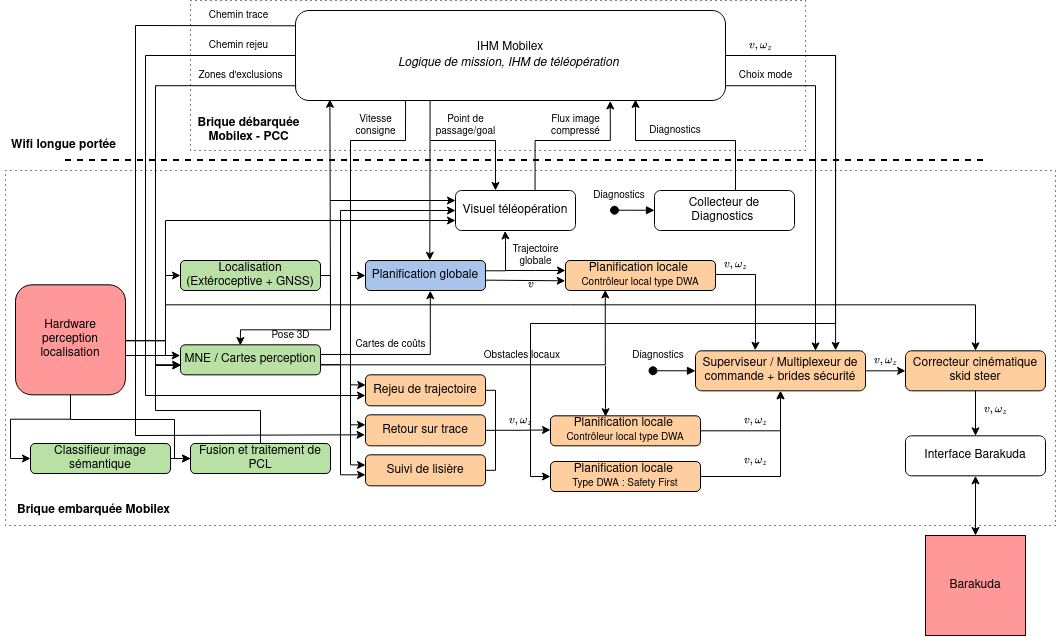
\includegraphics[width=1 \linewidth]{Corps_rapport/architecture_logicielle.png}
    \captionof{figure}{Diagramme synoptique de l'architecture logicielle du système}
    \label{fig13}
\end{center}

\subsection{Briques de perception de l'environnement}
Les briques de perception de l'environnement ont pour objectif de récolter des données provenant de capteurs majoritairement extéroceptifs pour pouvoir en concevoir une modélisation.

\subsubsection{Modèle Numérique d'Élévation}
La brique de cartographie selon un MNE (Modèle Numérique d'Élévation) se compose de deux parties : une librairie en C++ permettant de générer le MNE et un noeud ROS* permettant d'utiliser le MNE pour concevoir des cartes d'élévations correspondant aux modalités du Challenge.\\

\indent Le MNE permet de concevoir une représentation en vue de dessus de l'élévation de l'environnement sous la forme d'une carte de chaleur discrète (Figure \ref{fig14}) d'une résolution de 10x10cm. Il est construit à partir des données de position du robot, de ses vitesses 3D et des points LIDAR*. Ces données sont reçues de façon asynchrone et mises dans des tampons. Pour chaque nouvelle donnée, une partie de la carte, de 40x40m centrée autour de la position du robot, est publiée. Le MNE est mis à jour sur reception d'un scan LIDAR*, provoquant un ensemble d'interpolations pour trouver la vitesse et la position exacte du robot au moment exact du début du scan. Le nuage de points fourni par le LIDAR* est ainsi corrigé en distorsion en utilisant le début du scan comme référence et replacé dans le repère monde. Chaque point du nuage ainsi constitué sert alors à actualiser les valeurs d'élévations maximales présentes dans les tuiles de la carte grâce à un filtrage de Kalman* se servant de la position du robot et de la position des impacts LIDAR* et de leurs covariances associées.

\begin{center}
    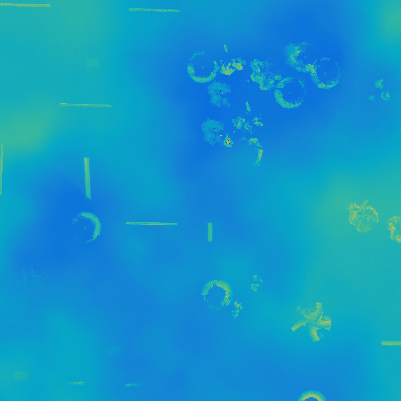
\includegraphics[width=0.4\linewidth]{Corps_rapport/MNE.png}
    \captionof{figure}{Extrait du Modèle Numérique d’Élévation sous forme d’une carte de chaleur}
    \label{fig14}
\end{center}
$\ $\

\indent Le noeud ROS* associé au MNE récupère la carte de 40x40m centrée autour du robot pour construire une carte de gradients, en utilisant un filtre de Sobel de taille 3x3 tuiles (30x30cm). Le Filtre de Sobel est un opérateur utilisé en traitement d'image pour faire de la détection de contours. Il permet de calculer le gradient d'intensité de chaque pixel ce qui indique la direction de la variation ainsi que son intensité, ce qui permet de faire ressortir les contours d'une image. En détournant cet usage sur notre carte d'élévation où la couleur nous donne une information sur la hauteur, on obtient une information sur les variations de hauteur pour chaque tuile.\\
\indent On vient ensuite seuiller notre carte de gradients afin d'obtenir une information correspondant aux différentes hauteurs d’obstacles à différencier pour le défi. La superposition de ces cartes permet d'obtenir une représentation des obstacles autour du robot comme illustré (Figure \ref{fig15}) :

\begin{center}
    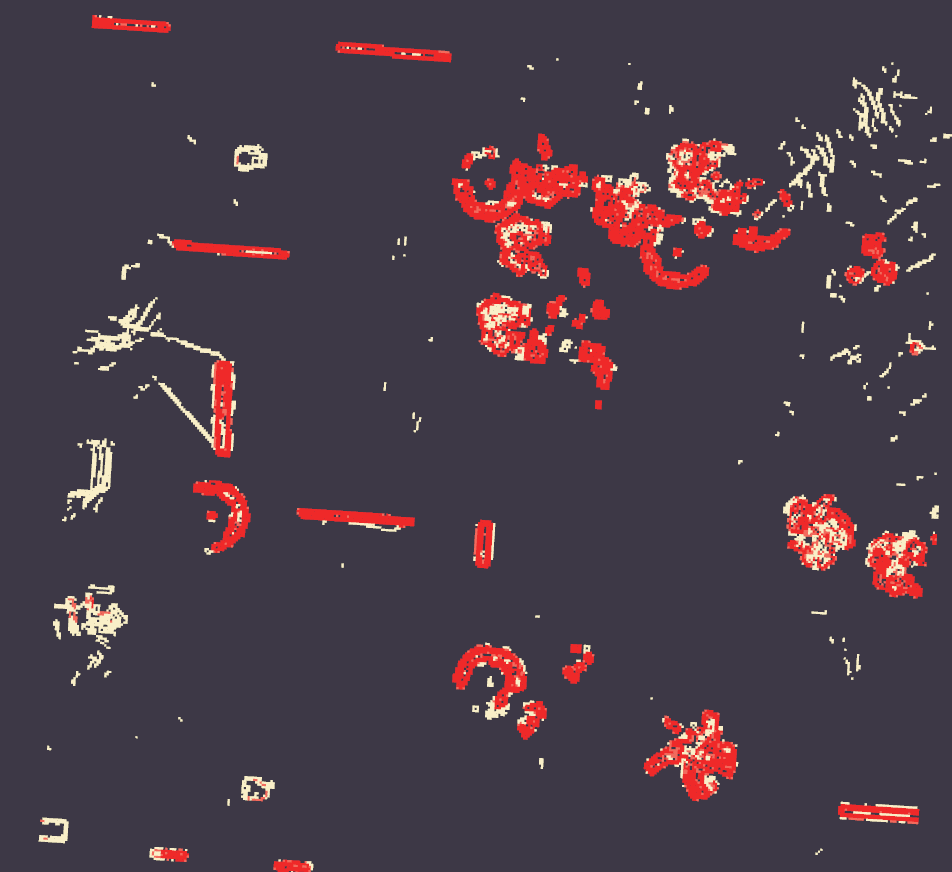
\includegraphics[width=0.4\linewidth]{Corps_rapport/Carte_obstacles.png}
    \captionof{figure}{Représentation des obstacles autour du robot}
    \label{fig15}
\end{center}
$\ $\

\indent Il est possible de demander une carte de coût associée à cette représentation selon un modèle client/serveur. Cette fonction est exploitée par le planificateur global lorsqu'il estime qu'un recalcul de la trajectoire globale est nécessaire.\\
\indent Il existe de nombreuses méthodes pour cartographier l'environnement \cite{thrun2009robotic}, permettant d'obtenir des représentations adaptées à la situation avec les capteurs disponibles \cite{lombard2020stochastic, jaspers2017multi, guerrero2015lidar}. La majorité de ces méthodes reposent néanmoins sur une fusion de données proprioceptives (odométrie, IMU) et extéroceptives (caméra, LIDAR*, ultrason, etc) avec un filtrage Kalman*.




%% verifier le maintien et la coherence de la section Segmentation d'image



\subsubsection{Segmentation d'image}
La brique de segmentation d'image* permet d'extraire des informations sémantiques à partir des images caméra. Elle a subi une modification complète par rapport aux années précédentes du défi. La combinaison des deux réseaux de neurones (détecteur open-set, YOLO World \cite{yoloworld2024} et un réseau de segmentation*, Efficient SAM \cite{efficientsam2024}) employée lors du défi 2 a été remplacée par un réseau de segmentation unique Segformer \cite{segformer}.\\


\begin{comment}
\indent Le détecteur open-set YOLO World est un réseau de neurones qui prend en entrée une image ainsi qu'un texte décrivant l'objet à détecter et à localiser. Il fournit en sortie des boîtes englobantes représentant les zones où les objets ont été détectés.\\\\
\indent Ce détecteur est dit open-set car, contrairement aux autres modèles YOLO, il est capable de détecter des objets qui ne figuraient pas dans son jeu de données d'entraînement initial. Cela est rendu possible grâce à l'intégration de techniques avancées d'apprentissage automatique et de traitement du langage naturel, permettant au modèle de comprendre et d'interpréter une large gamme d'objets à partir de descriptions textuelles.\\\\
\indent Une fois les objets détectés dans l'image, la sortie de YOLO World est utilisée comme entrée pour Efficient SAM, une version optimisée pour l'embarqué du réseau de neurones SAM \cite{segmentanything2023}. Efficient SAM se charge de segmenter précisément les objets en coloriant les pixels au sein des boîtes englobantes, ce qui nous donne le résultat (\hyperref[fig16]{Figure 16}) : \\
\begin{center}
    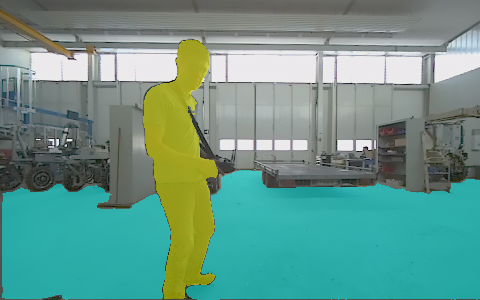
\includegraphics[width=0.8 \linewidth]{Corps_rapport/segmentation.png}
    \captionof{figure}{Résultat de la segmentation obtenu avec la combinaison de YOLO World et Efficient SAM}
    \label{fig16}
\end{center}
$\ $\

\indent Pour assurer un fonctionnement en temps réel, ces réseaux sont optimisés en supprimant les poids dont la valeur est proche de zéro, réduisant ainsi le nombre de paramètres. Cette optimisation est réalisée avec TensorRT. Une optimisation plus performante également envisagée serait d'utiliser des réseaux de neurones plus précis comme SAM et de réaliser une distillation de connaissances en entraînant un réseau de neurones constitué de moins de paramètres et spécialisé pour notre cas d'application à l'aide des sorties du réseau plus important.\\\\

\end{comment}

\indent SegFormer est une architecture de réseau de neurones dédiée à la segmentation sémantique d'images. À partir d'une image en entrée, il génère une carte de segmentation attribuant chaque pixel à une classe spécifique — dans notre cas : sol, hautes herbes et eau. Le réseau a d'abord été pré-entraîné sur le jeu de données public COCO, qui regroupe une large variété d'images annotées, puis affiné (fine-tuning) sur une base de données d'images propriétaires du groupe MOBITER. Ces données ont été acquises via la caméra ZED du robot lors de campagnes de collecte (ciblant les hautes herbes traversables et les flaques d'eau) réalisées sur les sites INRAE d'Aubière et de Montoldre.\\

\indent L'objectif est de fusionner cette information sémantique (sol, hautes herbes et eau) dans la brique du Modèle Numérique d'Environnement (MNE) pour ajouter une notion de traversabilité aux obstacles haute herbes et eau de la carte en mode dégradé. Et ainsi répondre aux exigences du défi 3.










\subsection{Briques de planification}
L'objectif des briques de planification est de calculer une trajectoire à suivre pour remplir un objectif à partir de la perception de l'environnement.

\subsubsection{Planification globale}
La brique de planification globale se sert des cartes de coûts générées par la brique du MNE pour recalculer périodiquement un chemin continu reliant le robot à un point dans le repère monde. Le chemin est obtenu par un algorithme de recherche de chemin classique de type A* \cite{hart1968formal} modifié.\\

\indent Cet algorithme est une amélioration de l'algorithme de Dijkstra \cite{dijkstra1959note} qui permet de trouver le chemin optimal selon un critère donné dans un graphe. \\

\indent Pour trouver ce chemin, l'algorithme de Dijkstra attribue à son noeud de départ un coût de 0 et attribue aux chemins vers les noeuds voisins des poids, par exemple la distance à vol d'oiseau. Le coût d'un noeud voisin correspond à la somme entre le coût du noeud précédent et le poids du chemin pour rejoindre le nouveau noeud (équation \eqref{eq1}).

\begin{equation} \label{eq1}
    c(n)=c(k)+p(k,a)
\end{equation}

où $n$ est le noeud exploré, $k$ est le noeud précédent et $a$ est l'action de déplacement utilisée depuis le noeud $k$.\\

\indent Il explore alors le noeud dont le coût est le plus faible en ajoutant les poids des chemins voisins ainsi que le coût des noeuds voisins et répète l'exploration jusqu'à atteindre l'objectif.\\

\indent La Figure \ref{fig17} est une représentation étape par étape de l'exploration d'une carte par l'algorithme de Dijkstra. Seuls les mouvements (haut, bas, gauche, droite) sont admissibles. La case bleue est le point de départ de l'algorithme, la case verte l'objectif à atteindre et le cercle jaune le noeud en cours d'exploration :

\newpage

\begin{figure}[h]
    \centering
    \begin{subfigure}[b]{0.48\textwidth}
        \centering
        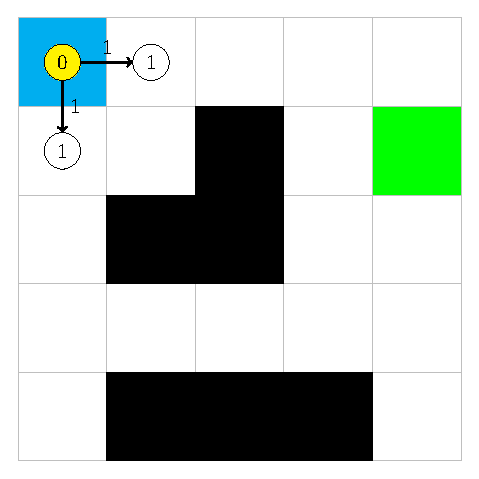
\includegraphics[width=\textwidth]{Corps_rapport/plan1.pdf}
        \caption{Exploration du noeud de départ}
        \label{fig:image1}
    \end{subfigure}
    \hfill
    \begin{subfigure}[b]{0.48\textwidth}
        \centering
        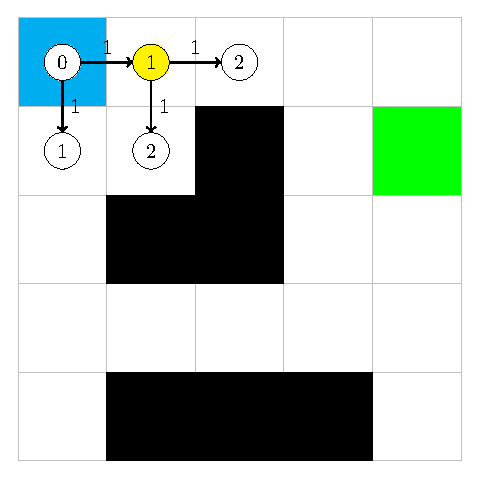
\includegraphics[width=\textwidth]{Corps_rapport/plan2.pdf}
        \caption{Exploration du noeud de coût le plus faible}
        \label{fig:image2}
    \end{subfigure}
    \vfill
    \begin{subfigure}[b]{0.48\textwidth}
        \centering
        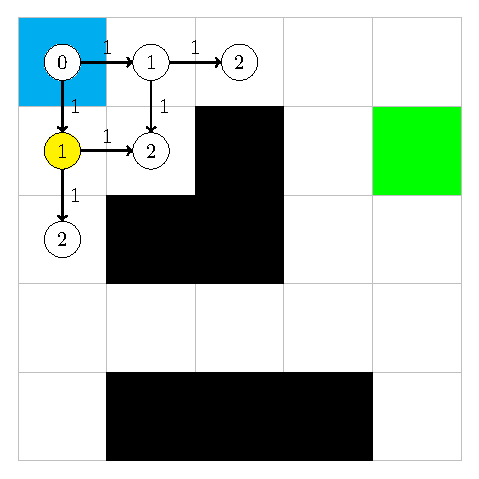
\includegraphics[width=\textwidth]{Corps_rapport/plan3.pdf}
        \caption{Nouvelle exploration}
        \label{fig:image3}
    \end{subfigure}
    \hfill
    \begin{subfigure}[b]{0.48\textwidth}
        \centering
        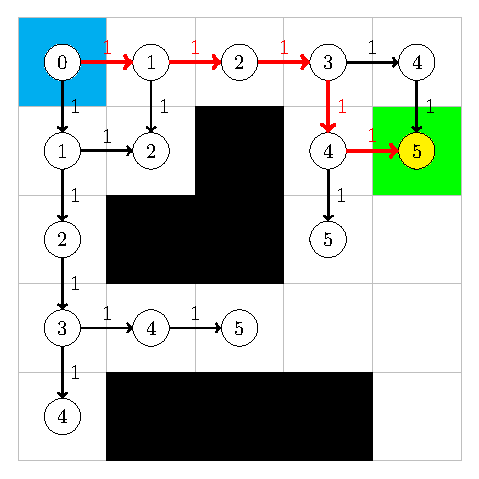
\includegraphics[width=\textwidth]{Corps_rapport/plan4.pdf}
        \caption{Résultat de l'exploration de la carte}
        \label{fig:image4}
    \end{subfigure}
    \caption{Fonctionnement de l'algorithme de Dijkstra}
    \label{fig17}
\end{figure}

\indent Face au probleme d'exploration aveugle (brute-force) dont fait face l'algorithme de Dijkstra, l'amélioration apportée par l'algorithme A* est d'ajouter un terme appelé l'heuristique dans le coût d'un noeud qui fournit une estimation du coût pour rejoindre l'objectif depuis ce noeud.\\
\indent Le coût utilisé lors de la sélection du noeud à explorer suit alors l'équation \eqref{eq2} :\\

\begin{equation} \label{eq2}
    f(n)=c(n)+h(n)
\end{equation}

où $c(n)$ est la somme des poids pour atteindre le noeud $n$ (comme dans l'algorithme de Dijkstra) et $h(n)$ est l'heuristique ajoutée pour aiguiller l'exploration vers l'objectif.\\

\indent Cette modification provoque une exploration plus rapide du graphe dès lors que l'heuristique est correctement choisie. Ce qui entrainne une reduction de la charge computationnelle dans le temps, ainsi qu'une plus faible mobilisation et consommation de ressources.\\
\indent Dans notre cas, l'heuristique est la distance à vol d'oiseau entre le noeud et l'objectif tandis que le poids entre deux noeuds est une somme entre la distance parcourue, un critère sur la similitude par rapport à la planification précédente sur les premiers mètres du chemin (afin d'éviter des oscillations) et un critère pondéré lié à la carte de coût du MNE. Le niveau de risque acceptable par le robot peut ainsi être choisi en modifiant la pondération de ce dernier coût, une faible pondération impliquant un chemin pouvant plus se rapprocher des obstacles détectés.\\
\indent La carte de coût utilisée (Figure \ref{fig18}) est similaire à une CostMap de ROS*, avec une zone critique définie autour de chaque obstacle correspondant aux zones où l'on considère que le robot va entrer en collision, une zone de danger où l'on considère que selon l'orientation le robot peut entrer en collision et un champ de potentiel décroissant avec la distance à l'obstacle.

\begin{center}
    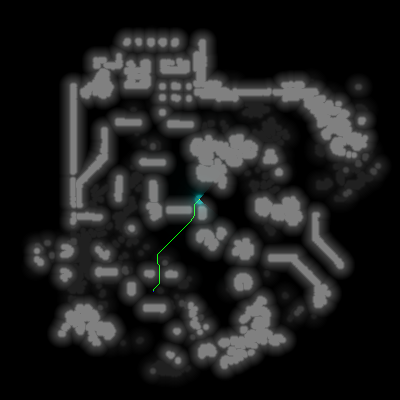
\includegraphics[width=0.4 \linewidth]{Corps_rapport/costmap.png}
    \captionof{figure}{Carte de coût utilisée par la planification globale}
    \label{fig18}
\end{center}

\indent Les zones critiques sont par définition impossibles à traverser tandis que les zones de dangers sont fortement pénalisées car il peut y avoir collision selon l'orientation du robot et sont donc souvent considérées uniquement lorsqu'il n'y a pas de solution alternative. Etant donné le manque de prise en compte de l'orientation du robot et l'absence de prise en compte de son modèle d'évolution, les chemins traversant des zones de danger pourraient ne pas être valides au sens de la traversabilité mais la brique de contrôle en aval, la planification locale, qui elle prend en compte l'orientation et l'enveloppe réelle (rectangulaire) du robot peut quand même trouver une solution à partir de ce chemin. Le surcoût computationnel qui interviendrait si l'on modifiait la carte de coûts en fonction de l'orientation du robot a encouragé à choisir ce compromis, en sachant que seuls les premiers mètres du chemin nous intéressent pour trouver une direction de déplacement privilégiée.\\
\indent Les algorithmes de Dijkstra et A* fournissent une solution optimale pour la situation donnée : carte échantillonnée et heuristique donnée pour l'A*. Il existe d'autres algorithmes de planification permettant de s'affranchir de la limitation de l'échantillonnage et permettant d'explorer l'environnement plus rapidement en générant des noeuds aléatoirement dans la carte et en essayant de les relier pour former un chemin jusqu'à l'objectif comme la Probalistic RoadMap \cite{prm1996}, le RRT \cite{rrt2000} et le RRT* \cite{rrtstar2011}. Les chemins générés ne sont plus optimaux et peuvent ne pas fournir de solution alors qu'il en existe une du fait du caractère aléatoire mais permettent de générer des chemins pouvant tenir compte de la cinématique du robot en appliquant une règle particulière lors de la génération des noeuds.

\subsubsection{Suivi de lisière}
Le suivi de lisière se compose de deux modules séquentiels : un module de détection des lisières issu de l'INRAE \cite{deremetz} et un module de suivi des lisières détectées.\\
\indent Le module de détection prend en entrée la carte de gradients seuillée pour les obstacles infranchissables fournie par le MNE, représentant une carte d'occupation 2D (carte encodant la présence d'obstacles, de manière probabiliste ou binaire), et donne en sortie au maximum deux lisières, une à gauche et une à droite. Il génère ensuite une trajectoire associée à une des deux lisières, en fonction du choix de l’utilisateur (suivre la lisière de droite ou de gauche) et l'envoie au module de suivi pour le calcul des commandes et leur envoi à la brique de supervision.\\
\indent La méthode de détection active de lisière implémentée repose sur l'adaptation de la détection de forme Snake contour et l'algorithme « Ball-Pivoting ». Cette approche permet de capturer uniquement les contours extérieurs des structures les plus proches du robot. La carte d'occupation peut avoir une certaine épaisseur pour des structures non "pleines", comme une haie clairsemée. Dans ce cas, extraire uniquement le contour extérieur permet d'éviter le traitement des points internes et de prévenir l'influence de points d'arrière-plan plus denses.\\
\indent L’algorithme de détection commence par la détection du départ de la lisière à gauche et à droite du robot. Pour cela, on translate un cercle jusqu’à ce que celui-ci intersecte un point. Ce point correspond au premier point de la lisière (Figure \ref{fig19}) :\\

\begin{center}
    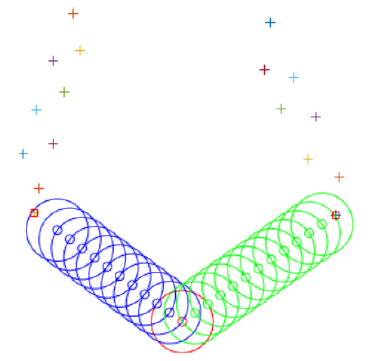
\includegraphics[width=0.3\linewidth]{Corps_rapport/lisiere1.png}
    \captionof{figure}{Détection du premier point}
    \label{fig19}
\end{center}
$\ $\
\indent Ensuite, on fait pivoter le cercle pour capturer l'ensemble des points de contour de la lisière (Figure \ref{fig20}) :\\
 \begin{center}
    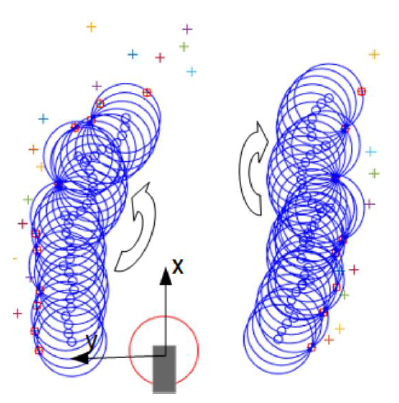
\includegraphics[width=0.3\linewidth]{Corps_rapport/lisiere2.png}
    \captionof{figure}{Détection du contour de la lisière}
    \label{fig20}
\end{center}
$\ $\
\indent Une fois les points de contour identifiés, des points intermédiaires sont ajoutés pour créer un nuage de points de chaque côté, formant une structure serpentine. Ces "serpents" représentent les bords estimés des lisières scannées (Figure \ref{fig21}) :\\
 \begin{center}
    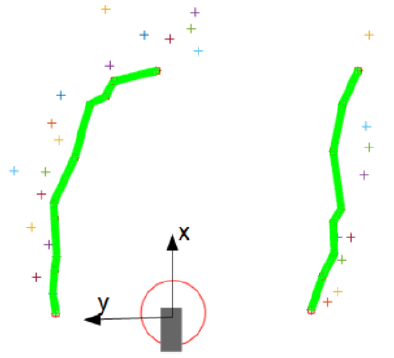
\includegraphics[width=0.3\linewidth]{Corps_rapport/lisiere3.png}
    \captionof{figure}{Création du "serpent" à partir des points de contacts du cercle et des points intermédiaires}
    \label{fig21}
\end{center}
$\ $\

\indent L’algorithme de détection de lisière est paramétrable. La taille du cercle a un grand impact sur la capacité de détection. Un cercle de petit diamètre permet d’obtenir un contour précis mais fonctionne mal avec les lisières naturelles qui possèdent de nombreuses aspérités. A l'inverse, un cercle de plus grande taille permet de passer au-dessus des aspérités et d’obtenir des lisières plus rectilignes. Les incréments de translation et de rotation du cercle sur le nuage de points permettent de maîtriser la précision du contour final. On peut également limiter la rotation du cercle sur le contour avec un angle maximal, afin d’éviter de détecter l’arrière de la lisière à la fin de cette dernière. Enfin, on limite la taille maximale du snake afin d’éviter des fausses détections et se concentrer sur la lisière en cours.\\
\indent Une fois les lisières détectées, elles sont décalées suivant leur direction normale moyenne et envoyées à l’algorithme de suivi comme trajectoires à suivre. Le module de suivi de trajectoire met en jeu un algorithme de suivi de chemin permettant une régulation latérale et longitudinale.\\
\indent La régulation latérale est réalisée par un correcteur Pure-Pursuit. Ce correcteur a pour objectif de calculer un taux de lacet à partir d'un arc de cercle reliant le centre du repère du robot à un point mobile P placé sur le chemin, en avance de phase du projeté orthogonal H du point O sur le chemin. Pour augmenter la stabilité de la régulation et réduire les oscillations à haute vitesse, le point de visée anticipée P est placé à une distance curviligne l du point H, où l est proportionnel à la vitesse de suivi.\\
\indent La régulation longitudinale est réalisée par un contrôleur qui détermine la vitesse de suivi en fonction de la vitesse consigne, de la distance à la fin du chemin et de la courbure du chemin en avance de phase. Cela permet de diminuer la vitesse à l'approche de virages ou de l'objectif.\\
\indent Cette régulation est implémentée comme une étape de minimisation d'un critère \eqref{eq3} formulé comme une somme pondérée du carré de la différence de vitesse à la vitesse de référence et de la moyenne de l'accélération centripète sur une portion du chemin à parcourir.\\
\begin{equation} \label{eq3}
    J(v)=\mu_1.(v_{max}-v)^2+\mu_2\frac{1}{n}\sum_{k=1}^n\frac{v^2}{R_{curv}(k)}
\end{equation}
$\ $\\
avec $v$ la vitesse à optimiser en $m.s^{-1}$, $v_{max}$ la vitesse de consigne en $m.s^{-1}$, $n$ le nombre de points de la portion de chemin et $R_{curv}(k)$ le rayon de courbure en $m$ du chemin au point k.\\

\indent Cette brique répondant parfaitement aux attentes du défi 2 qui ne prévoyait pas la présence d'obstacles sur le chemin, elle sera modifiée de manière à ce que le chemin de suivi de lisière généré s'adapte aux obstacles détectés par le MNE et que le robot puisse les contourner. Cette modification sera faite dans le cadre du défi 3.

\subsection{Briques de contrôle}
L'objectif des briques de contrôle est de retourner des commandes, ici de vitesses linéaires et angulaires, pour suivre un chemin donné en entrée en tenant compte de certains critères.

\subsubsection{Retour sur traces et rejeu de trajectoire}
Le retour sur traces et le rejeu de trajectoire sont assurés par la même brique, permettant d'enregistrer en temps réel la trajectoire du robot pour ensuite l'envoyer en entrée du même module de contrôle utilisé par le suivi de lisière avec un paramétrage spécifique pour fournir les commandes de déplacement à la brique de supervision.\\
\indent Pour assurer le déplacement dans un sens ou dans l'autre, il suffit d'inverser ou non les points du chemin, les consignes de vitesse et le cap du robot.







\subsubsection{Planification locale}
La planification locale se fait dans l’espace de la commande projetée en vue de dessus $(v_{2d},\dot{\alpha}_z)$, $v_{2d}$ étant la vitesse linéaire et $\dot{\alpha_z}$ la vitesse angulaire selon l'axe Z en 2D, en se servant de la carte de gradients seuillée pour les obstacles non franchissables.\\
\indent L’algorithme de planification utilisé est une adaptation de la Dynamic Window Approach (DWA) \cite{fox1997dynamic}. La méthode repose sur l'exploration de l'espace de commande afin de découvrir des combinaisons appropriées par la formulation d'un problème d'optimisation sur un horizon temporel glissant, plus étendu que l'intervalle de commande. L'avantage d'une telle approche pour la planification locale réside dans l'admissibilité cinématique des commandes tandis qu'une approche se limitant à l'espace de la tâche peut engendrer des chemins non praticables. Par exemple, l'utilisation de la planification donnée par le A* basée sur un environnement discrétisé et des champs de potentiels peut produire des inflexions abruptes dans un chemin qu'un robot non holonome ne peut suivre : le robot est incapable d'effectuer "un pas de côté" pour éviter un obstacle.\\
\indent D'autres alternatives de la DWA existent \cite{akmandor20203d, ozdemir2018follow} mais les recherches récentes tentent d'intégrer les contraintes de cinématique et la notion de risque directement dans la carte \cite{rummelhard2014probabilistic, laconte2021lambda, laconte2021novel, benrabah2023dual} ou d'utiliser l'apprentissage pour calculer les commandes optimales à exécuter \cite{hill2022online}. Cependant, ces algorithmes sont plus coûteux en temps de calcul.\\
\indent Des primitives de déplacement de type “arc” en vue de dessus (Figure \ref{fig22}) sont évaluées sur un horizon temporel de $2\ s$.  Chaque arc est paramétré par une paire de vitesses $(v_{2d},\dot{\alpha}_z)$ constantes sur la fenêtre temporelle.\\

\begin{center}
    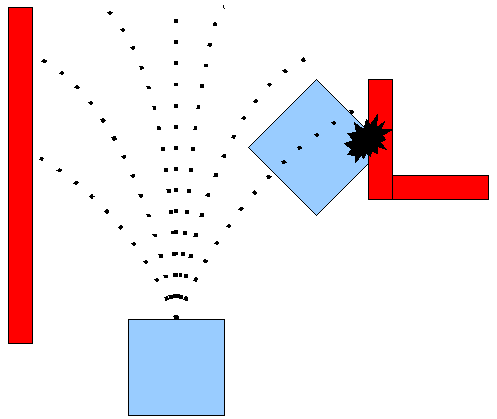
\includegraphics[width=0.3\linewidth]{Corps_rapport/DWA_illustration.png}
    \captionof{figure}{Illustration des trajectoires évaluées par la planification locale DWA}
    \label{fig22}
\end{center}


\begin{comment}
\indent Le principe de base de l'algorithme « Dynamic Window Approach » (DWA) est le suivant :\\
\begin{itemize}
\renewcommand{\labelitemi}{$\bullet$}
    \item Effectuer un échantillonnage discret dans l'espace de contrôle du robot (dx, dy, dtheta).
    \item Pour chaque vitesse échantillonnée, effectuer une simulation vers l'avant (\hyperref[fig22]{Figure 22}) à partir de l'état actuel du robot afin de prédire ce qui se passerait si cette vitesse était appliquée pendant une (courte) période.
    \item Évaluer (noter) chaque trajectoire résultant de la simulation vers l’avant, à l’aide d’un indicateur intégrant des caractéristiques telles que : la proximité des obstacles, la proximité de l’objectif, la proximité de la trajectoire globale et la vitesse. Écarter les trajectoires illégales (celles qui entrent en collision avec des obstacles).
    \item Choisir la trajectoire ayant obtenu le meilleur score et envoyer la vitesse associée à la base mobile.
    \item Répéter l’opération. \\
\end{itemize}
\end{comment}

\indent Le critère optimisé est un critère élaboré par SHERPA Engineering, fonction de l'écart par rapport à la vitesse consigne, de la direction / orientation du robot par rapport à l'objectif et de la présence d'obstacles. Il apparaît que selon la configuration d’obstacles, il n’y a aucune raison pour que ce critère soit convexe. \\
\indent Ce critère est optimisé avec une approche en force brute de type grid search: cette approche consiste à discrétiser l'espace de commande puis calculer le coût associé à chaque paire de commandes. La paire avec le plus faible coût étant la commande optimale pour la discrétisation donnée. Une fois la paire optimale trouvée, on calcule les commandes à envoyer au robot $(v,\omega_z)$ pour les adapter à la topologie du terrain dans le repère 3D.\\

\indent L'évaluation du terme de la présence des obstacles est lourd en calculs car il demande de générer l'empreinte du robot sur $2 s$ pour chaque paire de commandes. L'empreinte pour une paire de commande étant invariante, ces dernières sont générées en amont du lancement de la Brique MOBILEX* et stockées sous forme de LUT (Look-Up Tables). Lors du lancement de la brique de planification locale, elles sont chargées en mémoire vive, permettant de gagner un temps considérable pour trouver la commande optimale à appliquer. La superposition de l'empreinte et de la carte d'obstacles dans le repère du robot permet d'évaluer la présence d'obstacles sur la trajectoire générée.\\
\indent Une optimisation de cette brique à ete operée dans le cadre du defi 3. cette optimisation consiste à réduire la taille mémoire des LUT en ne stockant que les empreintes du robot à différentes orientations 








\begin{comment}

\subsubsection{Asservissement du taux de lacet}
\indent Le Barakuda est contrôlé en fournissant une consigne de vitesse identique aux roues d'un même côté, lui conférant ainsi une cinématique de type "skid steer". Avec ce type de cinématique, les roues avant et arrières dérapent nécessairement pour que le robot puisse tourner, contrairement à une cinématique à deux roues différentielles et une roue libre majoritairement employée en robotique indoor. Par conséquent, on ne peut pas faire l’hypothèse que le robot réalise vraiment le taux de rotation souhaité avec les vitesses de roue envoyées à gauche et droite en utilisant les équations d’un modèle cinématique différentiel à 2 roues sans glissement.\\\\
\indent Une solution simple et couramment employée pour résoudre ce problème consiste à asservir le taux de lacet pour que ce dernier corresponde bien aux commandes de haut niveau. Pour ce faire, on utilise les données odométriques fournie par le capteur INS pour obtenir le taux de lacet à tout instant. \\\\
\indent La correction implémentée est un simple correcteur Propotionnel Intégral avec un gain FeedForward. Le gain FeedForward joue le rôle d’un précompensateur trivial : inversion du gain $K = \lim_{\ s\ \rightarrow\ 0} H(s)$ où H est la fonction de transfert du système linéarisé. Le gain proportionnel fait l’essentiel de la régulation tandis que le gain intégral limite l’écart statique et l’effet des perturbations. Le gain feedforward augmente les performances en asservissement (précompensateur) en ramenant le système à un système à gain unitaire, tandis que le correcteur Proportionnel Intégral fait la régulation.\\\\
\indent Avec un modèle linéarisé $H(s)$ du Barakuda, il serait théoriquement possible 
d’augmenter les performances en régulation et ainsi réduire l’erreur de traînage (pour une consigne dynamique) sur le taux de lacet en remplaçant ce correcteur par un correcteur de type RST \cite{RST} que nous pourrions paramétrer pour obtenir un comportement souhaité de manière plus précise.

\end{comment}

\subsection{Autres briques}

\subsubsection{Interface avec le Barakuda}
Cette brique est responsable de la communication avec le Barakuda via des trames UDP. D’une part, elle fait remonter les informations provenant du robot au reste du système sous forme de diagnostics et, d’autre part, elle lui envoie les consignes de contrôle.

\begin{comment}
D’autre part, les consignes corrigées par le correcteur cinématique sont envoyées au robot, selon les formules habituelles \eqref{eq4} :\\

\begin{equation} \label{eq4}
    \Omega_{roues}=S\left(v_x\pm\omega_z\frac{L}{2}\right)
\end{equation}
$\ $\\
avec $\Omega_{roues}$ la vitesse de rotation des variateurs en $rpm$, $v_x$ la vitesse linéaire souhaitée en $m.s^{-1}$, $\omega_z$ la vitesse angulaire souhaitée en $rad.s^{-1}$, $L$ la voie (largeur) du véhicule en $m$ (ici, 0.95 m), et $S$ un facteur d’échelle dépendant des variateurs (ici, 1000 $rpm.s.m^{-1}$). 
\end{comment}

\subsubsection{Téléopération à la manette}
Cette simple brique lit et convertit les positions du joystick en commandes linéaires et angulaires avec un facteur d'échelle pour les envoyer directement au robot. L'ajout de la planification locale avec une configuration particulière entre cette brique et le robot permet de réaliser le mode safety first, empêchant le robot d'entrer dans des obstacles en modifiant légèrements les commandes problématiques transmises ou en arrêtant le robot.

\subsubsection{Brique de supervision}
Cette brique récupère l'ensemble des commandes fournies par les fonctions de pilotage et permet à l'opérateur de choisir laquelle est envoyée au robot via une liste déroulante dans l'IHM. Elle est également responsable d'une partie de la sécurité du robot puisqu'elle peut limiter la vitesse de ce dernier tout en gardant la même trajectoire lorsque la commande reçue provoque un dépassement du seuil de l'accélération centrifuge autorisé ou encore provoquer l'arrêt et le serrage des freins lors d'un dysfonctionnement grave retourné par une brique. La commande vérifiée ou limitée est ensuite envoyée au robot.

\subsubsection{Retour visuel annoté pour l'opérateur}
Cette brique utilise le retour image de la caméra frontale du système de perception pour y superposer différentes informations, éventuellement agrégées à partir des autres modules. \\
\indent Afin de respecter les exigences du challenge Mobilex*, les 
informations suivantes sont superposées au flux image : \\
\begin{itemize}
\renewcommand{\labelitemi}{$\bullet$}
    \item Affichage type “Viseur Tête Haute“ avec les angles de roulis, tangage, et lacet.
    \item Tracé des chemins de navigation trouvés par la planification globale en 3D.
    \item Tracé du chemin local à court terme (2 $s$), étant donné la commande actuelle.
    \item Représentation des obstacles avec des régions colorées en fonction de la distance.
    \item Representation colorée des flaques d'eau et végétation traversable 
    \item Représentation des waypoints en 3D dans l’image.
    \item Compas\\
\end{itemize}

\indent La projection dans l’image des informations définies dans le repère monde a été réalisée à l'aide de la calibration intrinsèque de la caméra ainsi que de la calibration extrinsèque caméra/LIDAR* réalisée auparavant et du système de transformations tf de ROS* permettant de définir une matrice de transformation homogène 4x4 pour projeter les éléments du repère monde vers le repère image. Cette transformation est utilisée pour la représentation des obstacles, des waypoints, des flaques d'eau, des végétations traversables et des chemins afin d'obtenir le retour annoté (Figure \ref{fig23}).

\subsubsection{IHM}
Enfin, la brique IHM fournit une interface graphique (Figure \ref{fig23}) sur le PC débarqué à l'aide du framework ROS* RQT. Elle permet au téléopérateur d'accéder au retour visuel annoté, d'envoyer des ordres de mission tout en ajustant les paramètres à sa guise, et d'enregistrer des trajectoires pour les modes « rejeu » et « retour sur traces ». Elle offre également la possibilité de saisir des coordonnées de points à atteindre, de consulter un ensemble de données et de diagnostics pour le débogage, ainsi que de définir et charger des paramètres pour les modes dégradés (hautes herbes, brouillard, etc.).

\begin{center}
    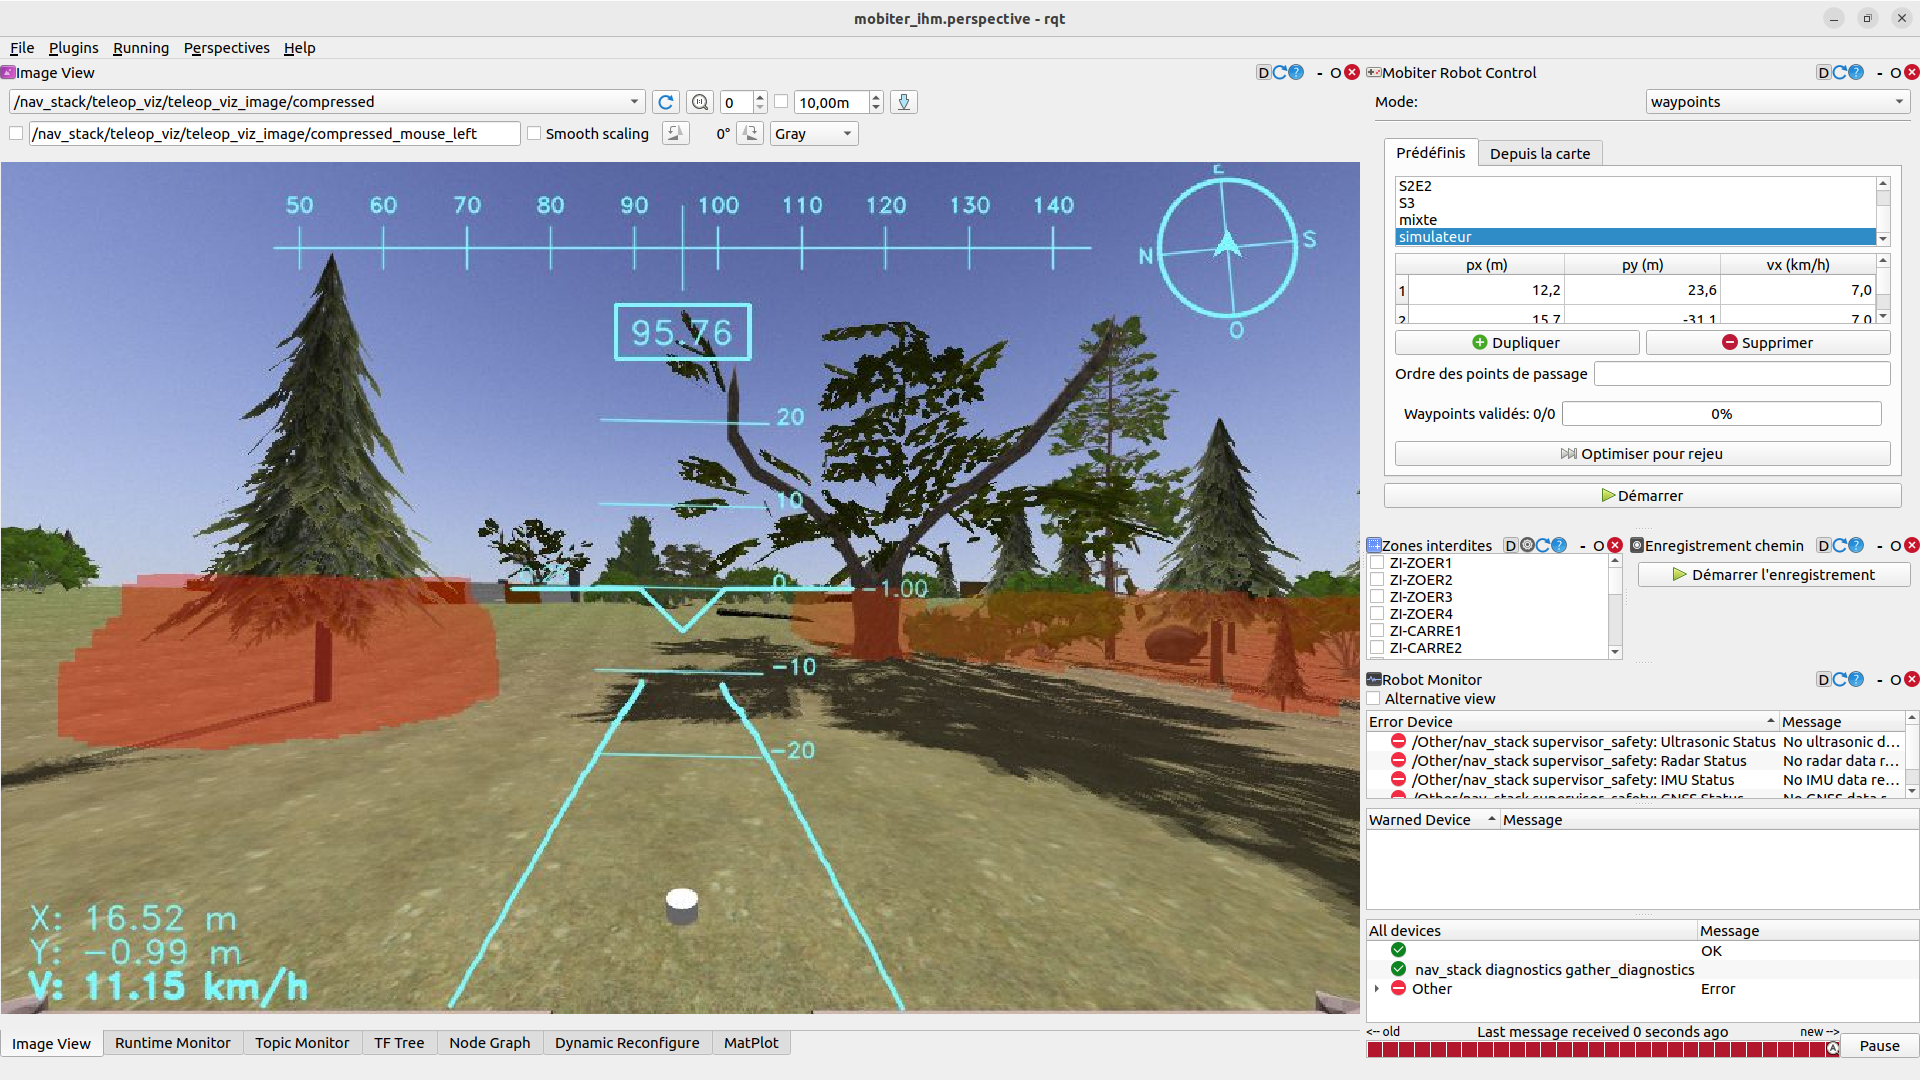
\includegraphics[width=0.9\linewidth]{Corps_rapport/rqt.png}
    \captionof{figure}{Interface RQT}
    \label{fig23}
\end{center}

\indent En parallèle de l'interface RQT, une visualisation RVIZ (Figure \ref{fig24}) peut être lancée. Elle permet d'afficher les différentes cartes générées par la brique MNE, d'observer les chemins planifiés et d'indiquer un point cible directement sur la carte. Une légende y est associée afin d'en faciliter la compréhension.

\begin{center}
    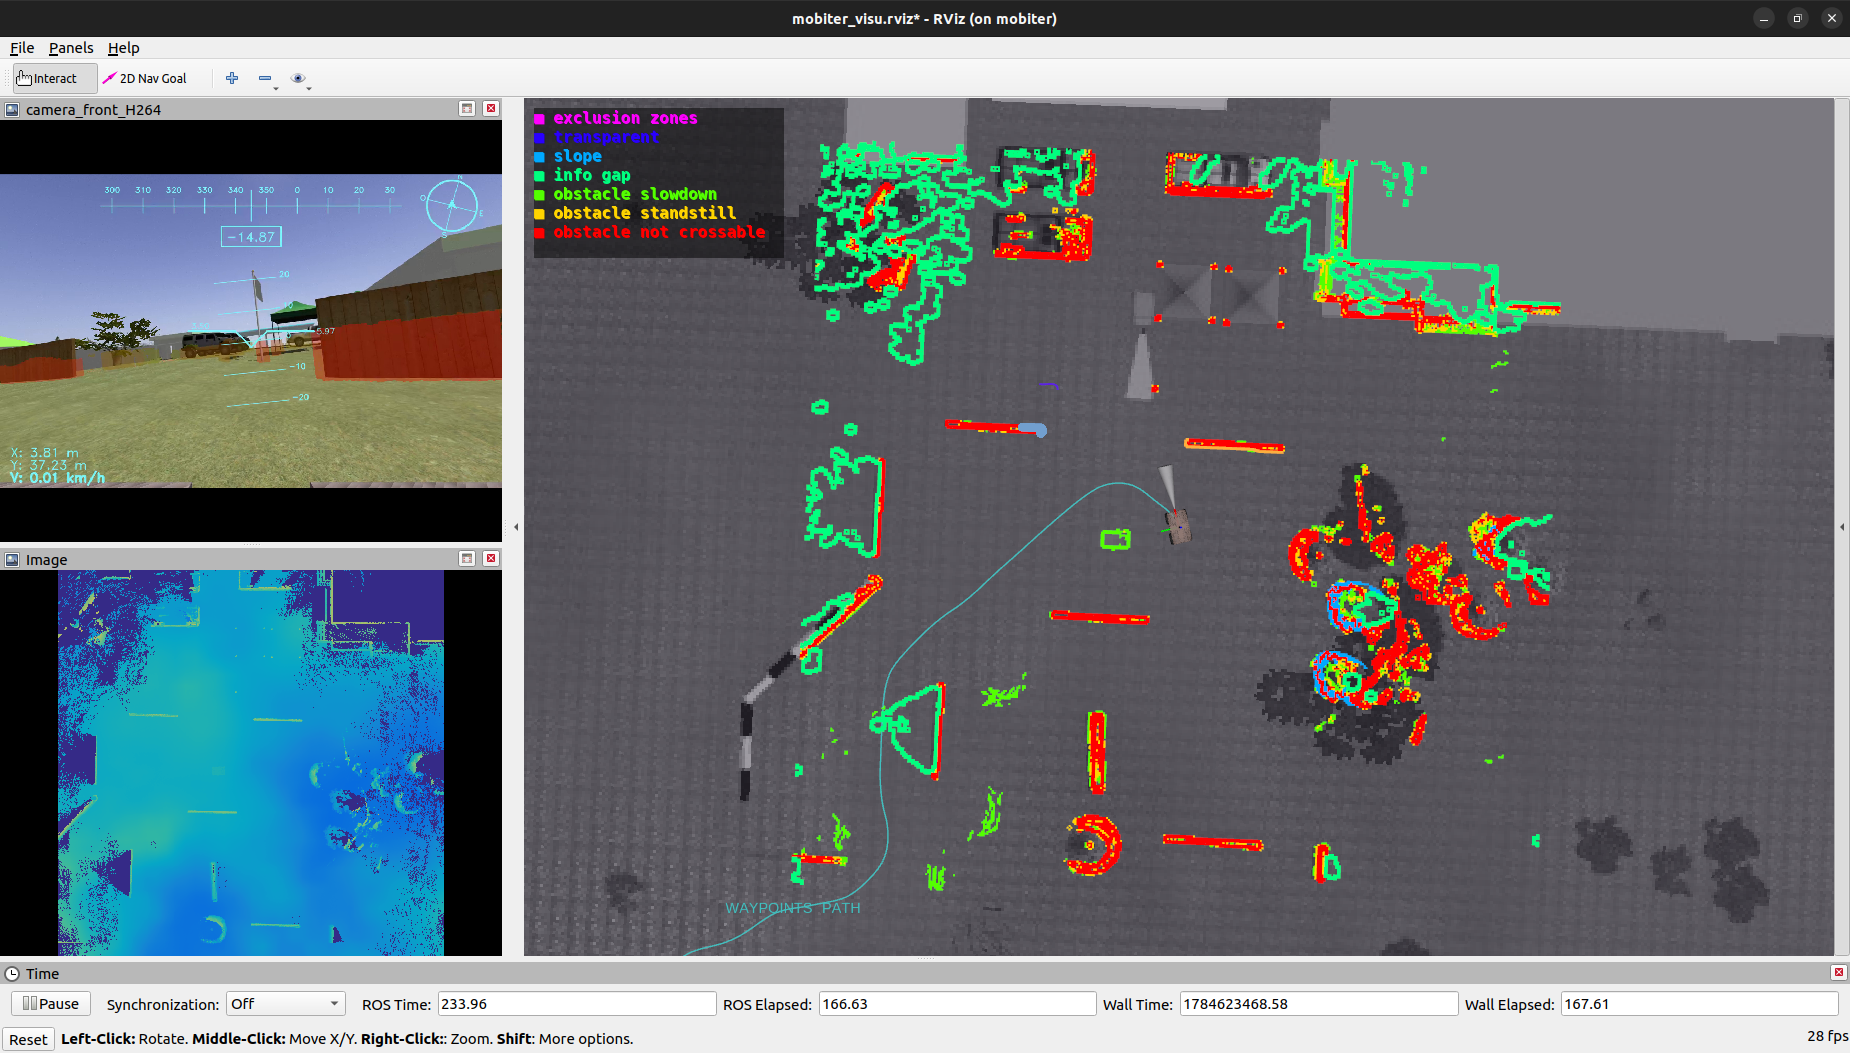
\includegraphics[width=0.9\linewidth]{Corps_rapport/rviz.png}
    \captionof{figure}{Visualisation RVIZ}
    \label{fig24}
\end{center}
